\documentclass{report}

% Language setting
% Replace `english' with e.g. `spanish' to change the document language
\usepackage[english]{babel}

% Set page size and margins
% Replace `letterpaper' with`a4paper' for UK/EU standard size
\usepackage[letterpaper,top=2cm,bottom=2cm,left=3cm,right=3cm,marginparwidth=1.75cm]{geometry}

%Code package
\usepackage{listings}
\lstdefinestyle{mystyle}{
    basicstyle=\ttfamily\footnotesize,
    breakatwhitespace=false,         
    breaklines=true,                 
    captionpos=b,                    
    keepspaces=true, 
    keywordstyle=\bfseries,
    commentstyle=\ttfamily,
    numbers=left,                    
    numbersep=5pt,                  
    showspaces=false,                
    showstringspaces=false,
    showtabs=false,                  
    tabsize=2,
    language=Python
}

\lstset{style=mystyle}
\lstset{language=Python}

% Useful packages
\usepackage{subcaption}
\usepackage[export]{adjustbox}
\usepackage{amsmath}
\usepackage{graphicx}
\usepackage{enumitem}
\usepackage[colorlinks=true, allcolors=blue]{hyperref}

\title{Progetto di Business Intelligence per i Servizi Finanziari}
\author{Banfi Michele 869294}

\begin{document}
\maketitle

\chapter{Sommario dei dati utilizzati}
\section{Titoli}
I titoli scelti per questo progetto sono i seguenti:

\noindent Settore tecnologico

Netflix, Inc. (\textbf{NFLX})

Meta Platforms, Inc. (\textbf{META})

\noindent La scelta di Netflix é stata basata sulle notizie di questi ultimi anni della perdita di utenti e del raggiungimento di utenti massimi che Netflix ha riscontrato e il conseguente calo del titolo sul mercato. Mentre Meta é stata presa in considerazione per il recente cambio di brand e nome, da Facebook a Meta, successivo al lancio del Metaverso

\noindent Settore finanziario

The Goldman Sachs Group, Inc. (\textbf{GS})

Citigroup Inc. (\textbf{C})

\noindent Le scelte di queste due aziende sono dovuto al loro andamento dopo un calo, infatti Goldman Sachs, dopo il calo del covid si é subito ripresa e ha raddoppiato il suo valore in meno di un anno. Mentre Citigroup dopo la crisi finanziaria del 2008 non ha mai raggiunto di nuovo i valori che aveva precedentemente

\noindent Settore consumer defensive

The Coca-Cola Company (\textbf{KO})

PepsiCo, Inc. (\textbf{PEP})

Coca-Cola e PepsiCo sono stati scelti in quanto concorrenti allo stesso mercato e in quando non hanno subito un calo dopo il covid-19 e inoltre, il loro andamento nel mercato sembra essere costante in rialzo.

\section{Scaricare i dati}
Per prima cosa importiamo le librerie che ci serviranno in questo progetto:
\begin{lstlisting}[language=Python]
    import pandas as pd
    import numpy as np
    import matplotlib.pyplot as plt
    import yfinance as yf
\end{lstlisting}
Procediamo al dowload dei dati tramite \lstinline{yfinance.download()}
\begin{lstlisting}[language=Python]
    start = "2012-11-30"
    end = "2022-11-30"

    #Tech
    NFLX = yf.download("NFLX", start, end)
    META = yf.download("META", start, end)

    #Financials
    GS = yf.download("GS", start, end)
    C = yf.download("C", start, end)

    #Consumers
    KO = yf.download("KO", start, end)
    PEP = yf.download("PEP", start, end)
\end{lstlisting}
\section{Fusione dei dati}
Ora procediamo alla fusione dei dati in un unico DataFrame e di ogni titolo prendiamo solo l'"Adj close".
\begin{lstlisting}[language=python]
    market = pd.concat([NFLX['Adj Close'], META['Adj Close'], GS['Adj Close'], C['Adj Close'], KO['Adj Close'], PEP['Adj Close']], axis=1)
    market.columns = ['NFLX', 'META', 'GS', 'C', 'KO', 'PEP']
\end{lstlisting}
\section{Presentazione dei dati}
Per mostrare la struttura del nostro DataFrame possiamo usare la seguente funzione che ci ritorna le righe iniziali del nostro DataFrame
\begin{lstlisting}[language=python]
    market.head()
\end{lstlisting}
\begin{tabular}{lrrrrrr}
\toprule
{} &       NFLX &       META &          GS &          C &         KO &        PEP \\
Date       &            &            &             &            &            &            \\
\midrule
2012-11-30 &  11.672857 &  28.000000 &   99.521103 &  28.667482 &  27.682371 &  52.271511 \\
2012-12-03 &  10.857143 &  27.040001 &  100.036469 &  28.377247 &  27.288162 &  52.018406 \\
2012-12-04 &  12.378571 &  27.459999 &   98.498741 &  28.435295 &  27.120255 &  52.010952 \\
2012-12-05 &  11.910000 &  27.709999 &   98.963432 &  30.234777 &  27.237057 &  52.301300 \\
2012-12-06 &  12.310000 &  26.969999 &   99.022560 &  30.699169 &  27.288162 &  52.533886 \\
\bottomrule
\end{tabular}

E inoltre possiamo procedere anche alla stampa di un grafico di questi dati:
\begin{lstlisting}[language=python]
    market.plot(grid=True, title="Markets Adjs Closes")
    market.plot(grid=True, title="Markets Adjs Closes", subplots=True)
\end{lstlisting}

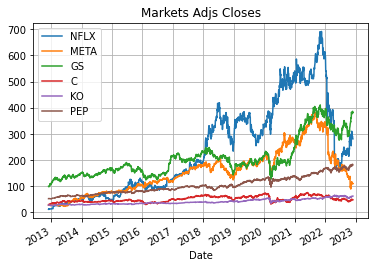
\includegraphics[width=0.5\textwidth, center]{market.png}

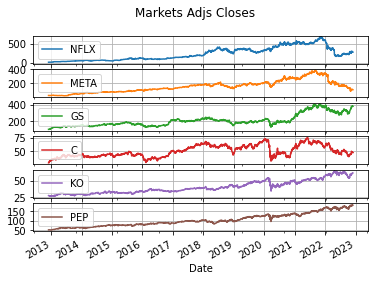
\includegraphics[width=0.5\textwidth, center]{marketSubplots.png}

\chapter{Statistiche descrittive}
\section{Rendimenti annauli}
Per calcolare il rendimento \textbf{composto} e \textbf{cumulato annuale} dobbiamo prima trasformare i dati da giornalieri ad annuali nel seguente modo:
\begin{lstlisting}[language=python]
    NFLXy = NFLX.groupby(pd.Grouper(freq='Y')).last()
\end{lstlisting}
Li raggruppiamo e li salviamo in \lstinline{marketY}.
Dopodiché possiamo procedere con il calcolo dei \textbf{rendimenti cumulati annui} e quello dei \textbf{rendimenti composti annui}:
\begin{lstlisting}[language=python]
    #Rendimento cumulato dei nostri titoli
    marketY2 = marketY.pct_change(1)
    marketY2 = marketY2.dropna()
    marketY3 = np.cumprod(marketY2 + 1)

    #Rendimento composto annuale NFLX
    rcoNFLXy = ((marketY['NFLX'][-1]/marketY['NFLX'][0])**(1/marketY['NFLX'].count()) - 1) *    100
\end{lstlisting}
Applichiamo questo procedimento per tutti i titoli.

\noindent Questo é il risultato dei nostri rendimenti cumulati:

\begin{tabular}{lrrrrrr}
\toprule
{} &       NFLX &      META &        GS &         C &        KO &       PEP \\
Date       &            &           &           &           &           &           \\
\midrule
2013-12-31 &   3.976347 &  2.052968 &  1.407936 &  1.318358 &  1.172331 &  1.246481 \\
2014-12-31 &   3.689491 &  2.930879 &  1.559786 &  1.370062 &  1.234067 &  1.461696 \\
2015-12-31 &   8.647370 &  3.931630 &  1.469481 &  1.314142 &  1.297496 &  1.589572 \\
2016-12-31 &   9.359542 &  4.321938 &  1.982669 &  1.523134 &  1.292863 &  1.713495 \\
2017-12-31 &  14.512582 &  6.628851 &  2.136010 &  1.934785 &  1.478803 &  2.018807 \\
\bottomrule
\end{tabular}

\section{Rendimenti semplici e logaritmici}
Usiamo le seguenti formule per calcolarci i \textbf{rendimenti semplici} e \textbf{logaritmici}
\begin{lstlisting}[language=python]
    #Rendimento semplice
    rsNFLX = NFLX['Adj Close'] / NFLX['Adj Close'].shift(1)
    #Rendimento logaritmico
    rlNFLX = np.log(NFLX['Adj Close'] / NFLX['Adj Close'].shift(1))
\end{lstlisting}
Applichiamo le stesse formule per tutti i titoli e li uniamo in un singolo DataFrame ottenendo i seguenti grafici

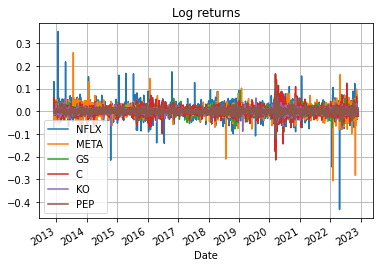
\includegraphics[width=0.5\textwidth, center]{logReturns.png}

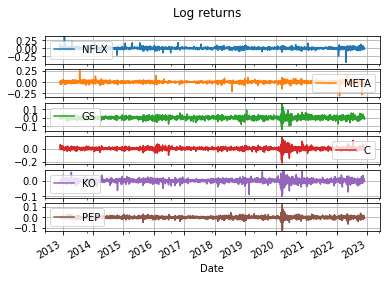
\includegraphics[width=0.5\textwidth, center]{logReturnsSubplots.png}

Possiamo subito notare come le serie dei rendimenti possano darci una diversa prospettiva sull'andamento dei titoli rispetto alla sola serie dei prezzi, infatti ci permettono di confrontare diversi titoli aventi prezzi molto differenti e quindi di concentrarci sull'andamento e non sul valore. Nel primo grafico Netlfix (blu) e Meta(arancione) sono i due titoli con piú outliers rispetto agli altri titoli e che di conseguenza hanno avuto dei movimenti di prezzo  piú ampi e forti (sia in positivo che in negativo) rispetto agli altri titoli. Inoltre nel secondo grafico si nota l'importanza che ha avuto la crisi causata dall'epidemia di covid-19 sui mercati nel 2020, tranne che nei che su Netflix e Meta. Che peró hanno avuto dei cali dopo il 2020, Netflix ad esempio aveva divulgato la notizia della perdita di abbonati alla piattaforma.
\section{Rendimenti con istogrammi}
Plottiamo ora i rendimenti tramite gli istogrammi con il seguente metodo:
\begin{lstlisting}
    plt.hist(rlNFLX, density=True, bins=50)
    plt.title('NFLX Logarithmic returns histogram')
\end{lstlisting}

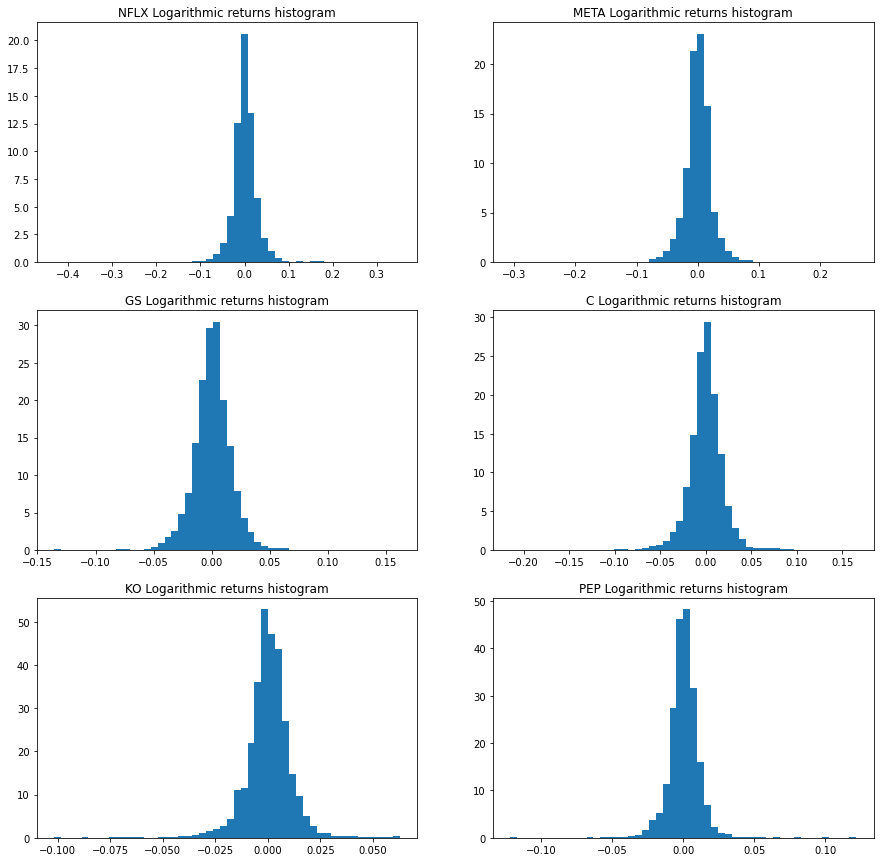
\includegraphics[width=0.5\textwidth, center]{logHist.png}
Tramite gli istogrammi possiamo valutare la quantitá di volte che si sono presentati i rendimenti nella serie, e si nota subito che per un titolo come Golden Sachs si ha un istogramma piú largo rispetto a Netflix ad esempio, questo indica una maggiore stazionarietá del titolo e di conseguenza dei cambi di prezzo piú lievi.
\section{Grafici diagnostici}
Per studiare meglio i rendimenti aggiungiamo altri 3 grafici all'istogramma, la kernel density, boxplot e qq-plot.
\begin{itemize}[leftmargin=30pt, rightmargin=2cm]
\item Box Plot \textrightarrow{} In un solo gradico ci mostra: mediana, media primo quartile, terzo quartile e la distanza tra essi, e infine ci mostra anche gli outliers
\item QQ-Plot \textrightarrow{} Ci mostra quanto una serie é prossima alla normalitá. Una serie normale ha la linea del qq plot esattamente in diagonale
\item Kernel density \textrightarrow{} É un grafico come l'istogramma, ma al posto che raggruppare i dati, li rappresenta tutti
\end{itemize}
Il codice per produrre i grafici é il seguente:
\begin{lstlisting}[language=python]
    #NFLX
    fig = plt.figure(figsize=(15, 15))

    ax=fig.add_subplot(221)
    plt.hist(rlNFLX, density=True, bins=50)
    plt.title('NFLX Log returns histogram')
    
    ax=fig.add_subplot(222)
    plt.boxplot(rlNFLX)
    plt.title('NFLX Log returns Boxplot')
    rlNFLX.to_frame().boxplot()
    
    ax=fig.add_subplot(223)
    sm.graphics.qqplot(rlNFLX, line='s', ax=ax)
    plt.title('NFLX Log returns Q-Q plot')

    ax=fig.add_subplot(224)
    rlNFLX.plot.density()
\end{lstlisting}
Il codice soprastante é il codice per produrre i grafici di Netflix, in modo equivalente possiamo produrre i grafici per gli altri titoli.
\subsection{NFLX}
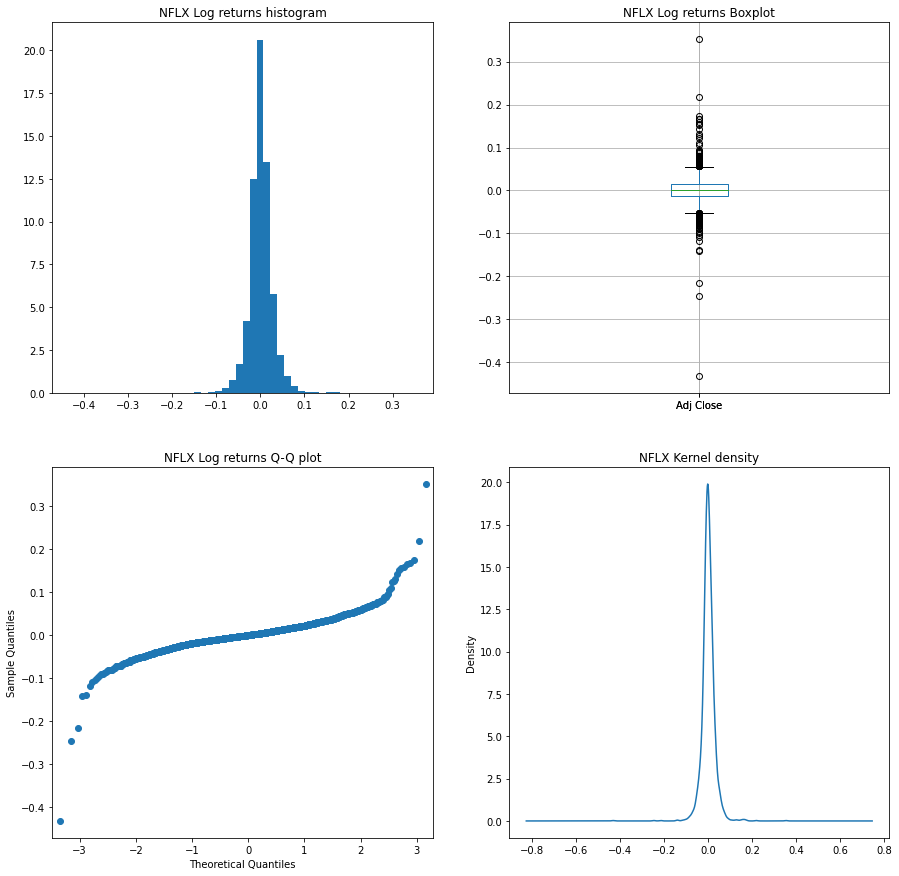
\includegraphics[width=0.5\textwidth, center]{graficiNFLX.png}
Netflix presenta una distribuzione molto compatta e ricca di outliers, come si puó vedere nel BoxPlot.
\subsection{META}
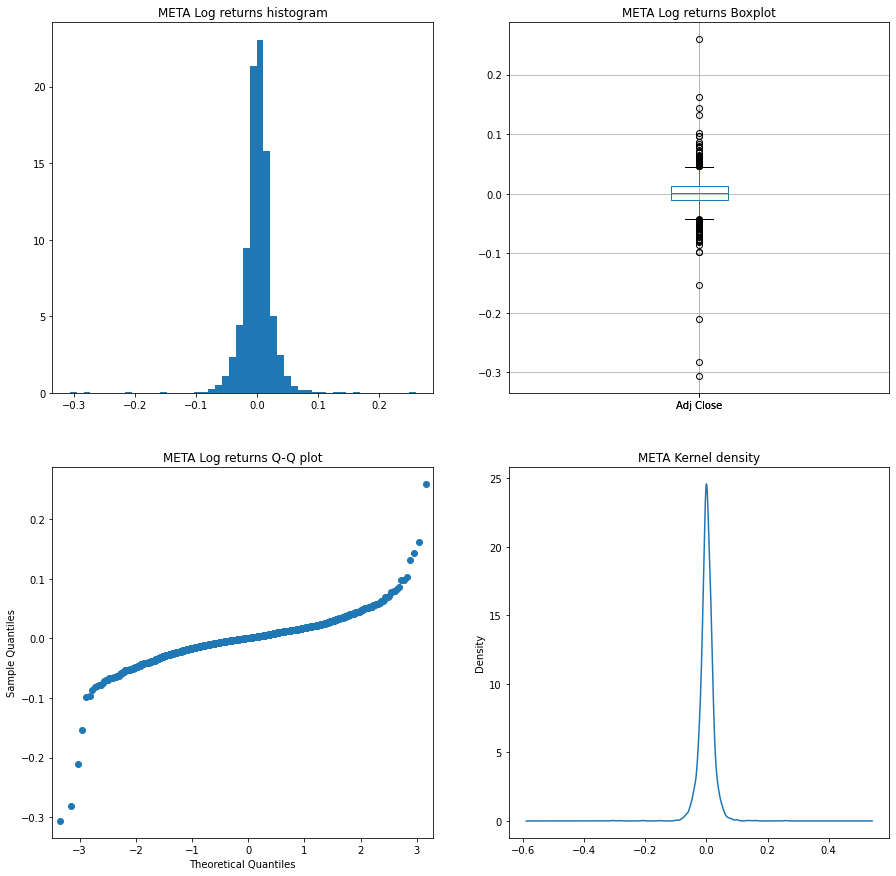
\includegraphics[width=0.5\textwidth, center]{graficiMETA.png}
Anche META resta molto distante dalla normalitá e resta comunque molto ricca di outliers, piú vicini peró alla media rispetto a NFLX.
\subsection{GS}
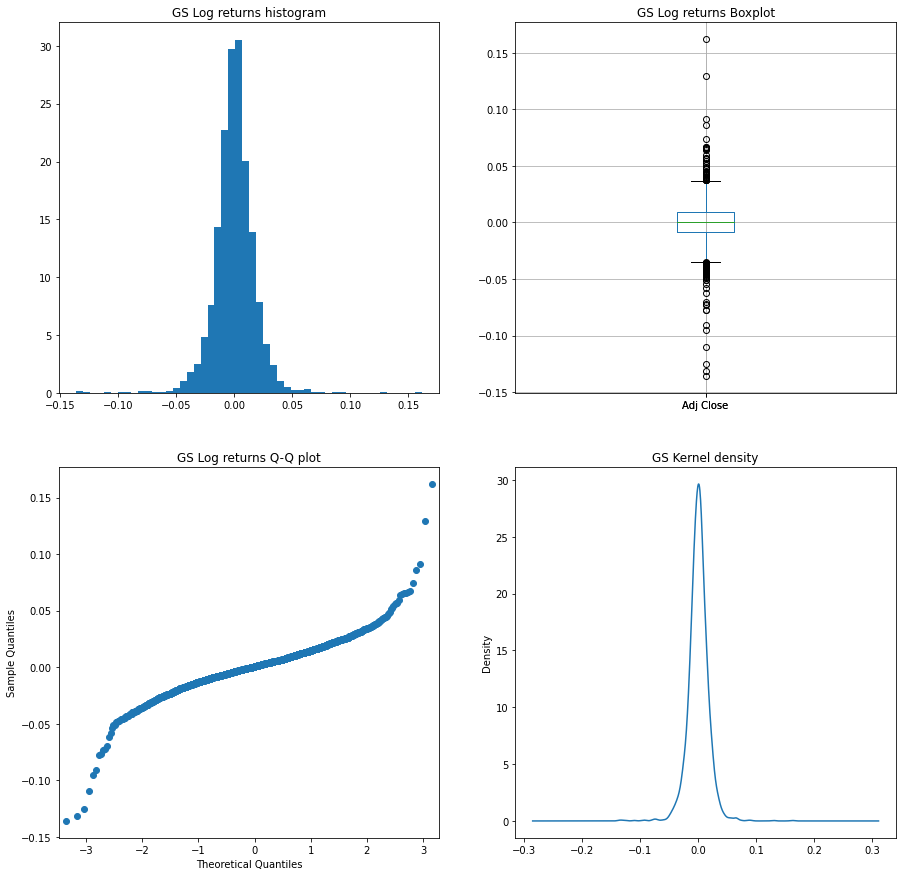
\includegraphics[width=0.5\textwidth, center]{graficiGS.png}
Goldach Sech é il titolo tra i sei che si avvicina leggermente un pó di piú alla normalitá ma ne resta comunque molto lontano.
\subsection{C}
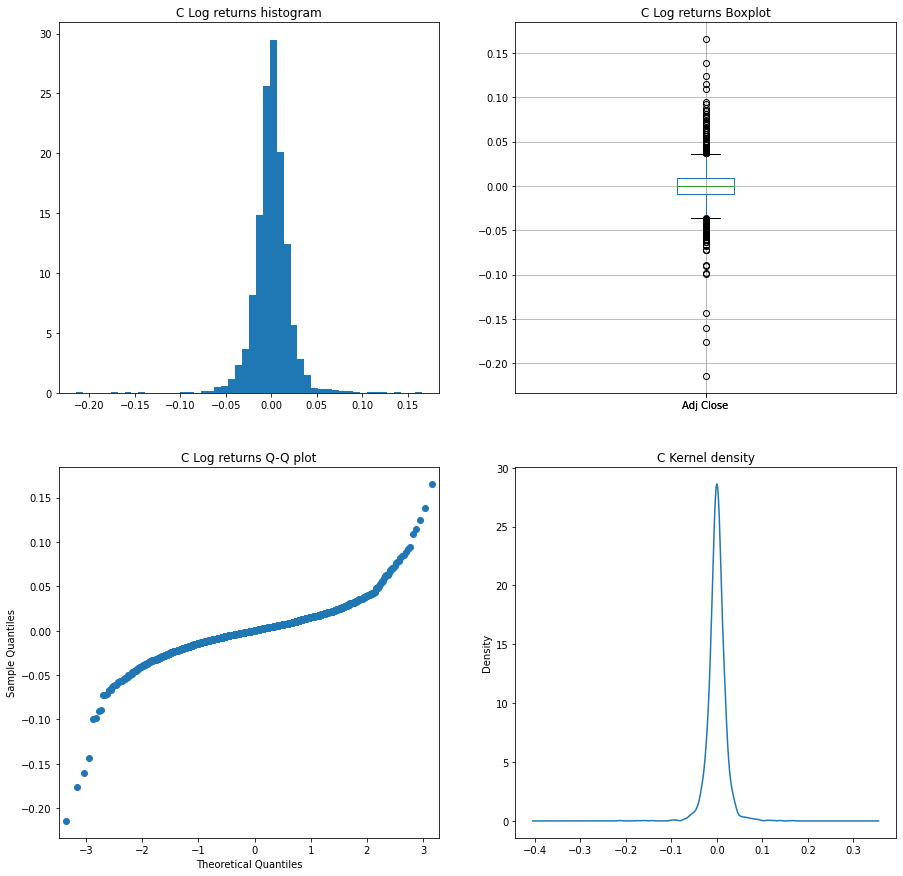
\includegraphics[width=0.5\textwidth, center]{graficiC.png}
Citigroup, come Netflix ha molti outliers distanti dalla media
\subsection{KO}
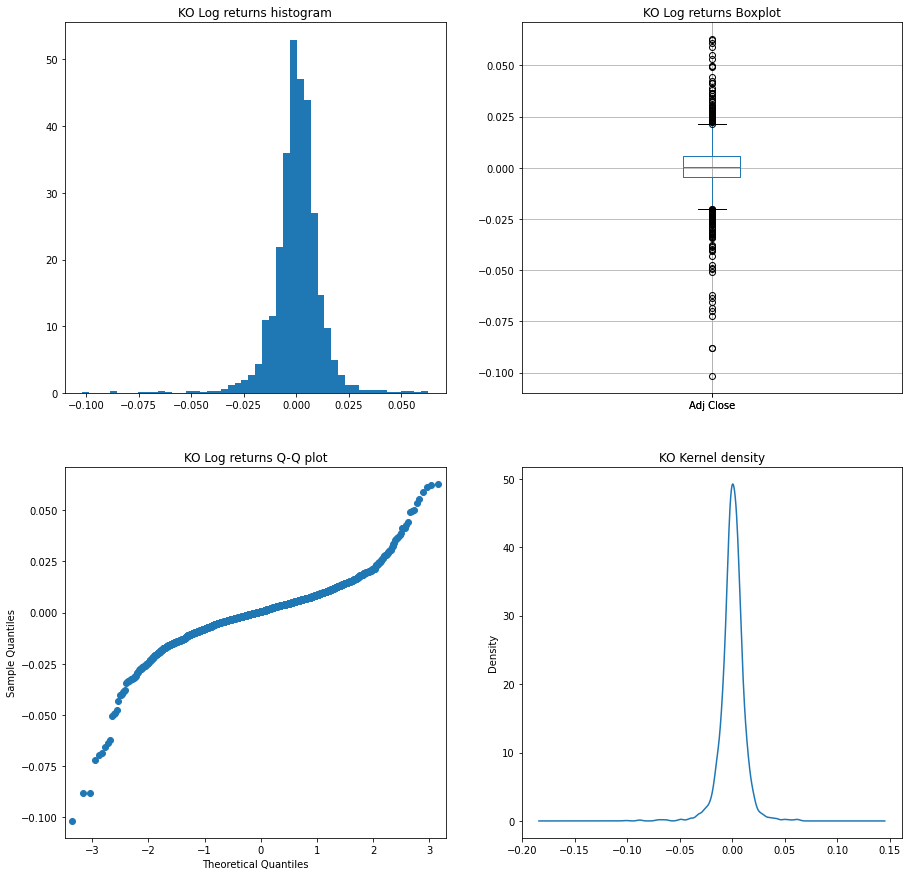
\includegraphics[width=0.5\textwidth, center]{graficiKO.png}
Anche Coca-Cola si avvicina a Goldman Sachs per vicinanza alla normalitá ma sempre rimanendo ricchissimo di outliers. E inoltre é la serie piú spostata rispetto al centro, quindi con una skewness maggiore
\subsection{PEP}
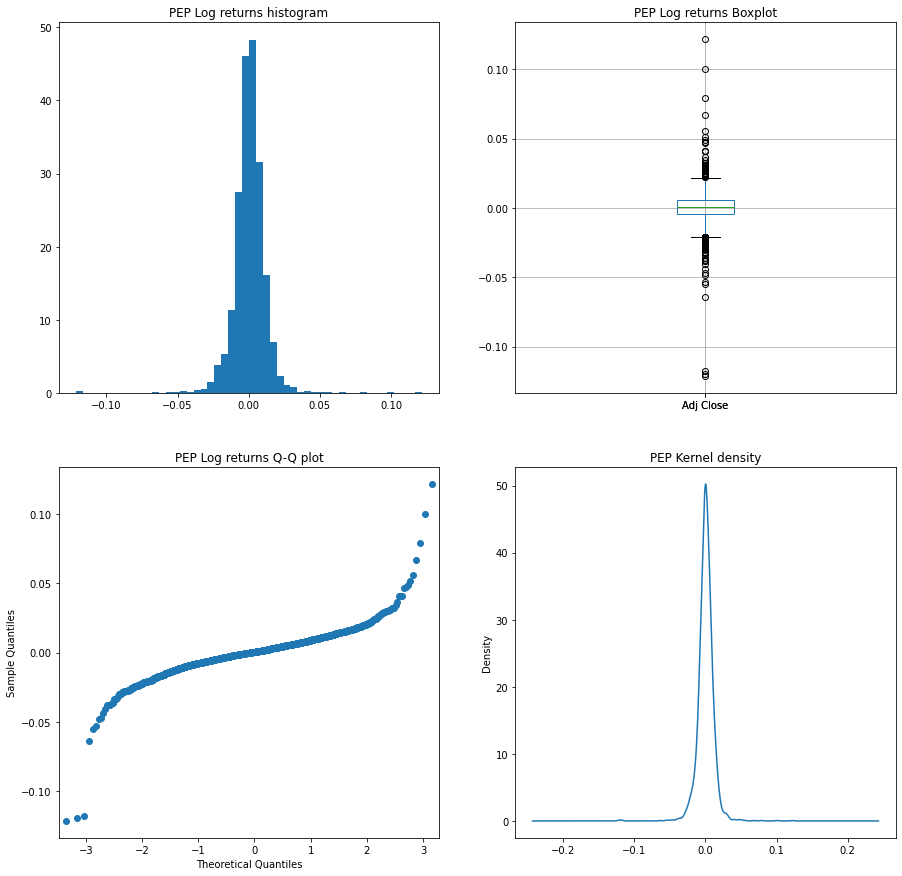
\includegraphics[width=0.5\textwidth, center]{graficiPEP.png}
Pepsi, rispetto al suo concorrente presenta la maggior parte dei suoi outliers vicini alla media e pochi lontani

\section{Statistiche descrittive univariate}
Ora procediamo con il calcolo dei seguenti dati:
\begin{itemize}[leftmargin=30pt, rightmargin=2cm]
\item Media
\item Varianza
\item Deviazione standard
\item Asimmetria
\item Curtosi
Per calcolare i dati usiamo le seguenti funzioni sulle serie:
\begin{lstlisting}[language=python]
    #NFLX
    meanNFLX = round(rlNFLX.mean(), 4)
    varNFLX = round(rlNFLX.var(), 4)
    stdNFLX = round(rlNFLX.std(), 4)
    skewNFLX = round(rlNFLX.skew(), 4)
    kurtNFLX = round(rlNFLX.kurtosis(), 4)
\end{lstlisting}
Calcolati tutti i valori li uniamo in un unico DataFrame cosi che possiamo confrontarli
\end{itemize}
\begin{tabular}{lrrrrrr}
\toprule
{} &     NFLX &     META &      GS &        C &       KO &      PEP \\
\midrule
Mean               &   0.0013 &   0.0005 &  0.0005 &   0.0002 &   0.0003 &   0.0005 \\
Variance           &   0.0009 &   0.0006 &  0.0003 &   0.0004 &   0.0001 &   0.0001 \\
Standard Deviation &   0.0300 &   0.0241 &  0.0176 &   0.0203 &   0.0115 &   0.0115 \\
Skewness           &  -0.4118 &  -1.1173 & -0.1999 &  -0.4763 &  -0.8931 &  -0.5869 \\
Kurtosis           &  31.0142 &  27.8449 &  9.8418 &  14.9718 &  10.6779 &  23.7351 \\
\bottomrule
\end{tabular}

\noindent Il titolo con il rendimento piú alto é Netflix che ha una media di \num{0.0013} mentre quello con il rendimento piú basso é Citigroup con \num{0.0002}.
Mentre per quanto riguarda la deviazione standard, il titolo piú alto é sempre Netflix con \num{0.03} mentre quelli piú bassi sono Coca-Cola e Pepsi con \num{0.0115} [...]
\section{Varianza e covarianza}
Calcoliamo ora la matrice di covarianza tra i nostri titoli con le seguenti funzioni:
\begin{lstlisting}[language=python]
    #Covariance Matrix
    covariance = rlMarket.cov().iloc[0,1]
    covarianceMatrix  = rlMarket.cov()
\end{lstlisting}
Che ci restituiscono per la covarianza: \num{0.0003}, mentre per la matrice:

\begin{tabular}{lrrrrrr}
\toprule
{} &      NFLX &      META &        GS &         C &        KO &       PEP \\
\midrule
NFLX &  0.000902 &  0.000298 &  0.000147 &  0.000157 &  0.000047 &  0.000068 \\
META &  0.000298 &  0.000583 &  0.000157 &  0.000164 &  0.000062 &  0.000082 \\
GS   &  0.000147 &  0.000157 &  0.000311 &  0.000296 &  0.000085 &  0.000084 \\
C    &  0.000157 &  0.000164 &  0.000296 &  0.000414 &  0.000102 &  0.000092 \\
KO   &  0.000047 &  0.000062 &  0.000085 &  0.000102 &  0.000131 &  0.000096 \\
PEP  &  0.000068 &  0.000082 &  0.000084 &  0.000092 &  0.000096 &  0.000132 \\
\bottomrule
\end{tabular}

Procediamo con il calcolo della matrice di correlazione con il seguente codice:
\begin{lstlisting}
    correlation = rlMarket.corr()
    plt.figure(figsize=(15,15))
    plt.title('Matrice di correlazione')
    sns.heatmap(correlation, vmax=1, square=True, annot=True, cmap='YlGnBu')
\end{lstlisting}

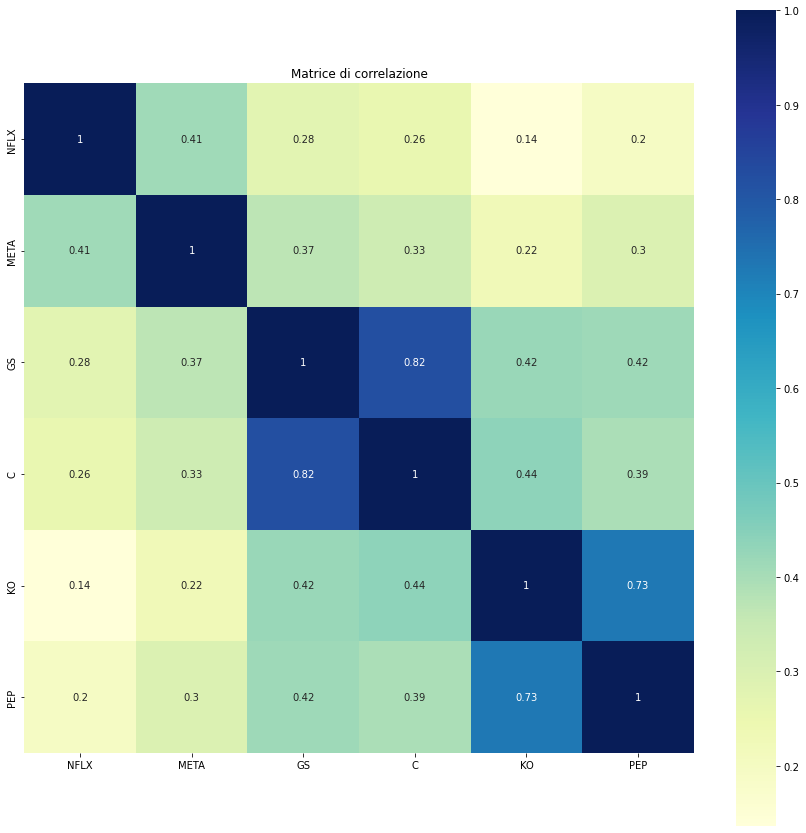
\includegraphics[width=0.5\textwidth, center]{correlationMatrix.png}
Possiamo notare che i titoli dello stesso settore sono molto correlati, in particolare GS e C piú degli altri

Proseguiamo quindi con la costruzione degli scatter plot
\begin{lstlisting}
    plt.figure(figsize=(15,15))
    pd.plotting.scatter_matrix(rlMarket, figsize=(12, 12))
    plt.show()
\end{lstlisting}
Con la seguente immagine:

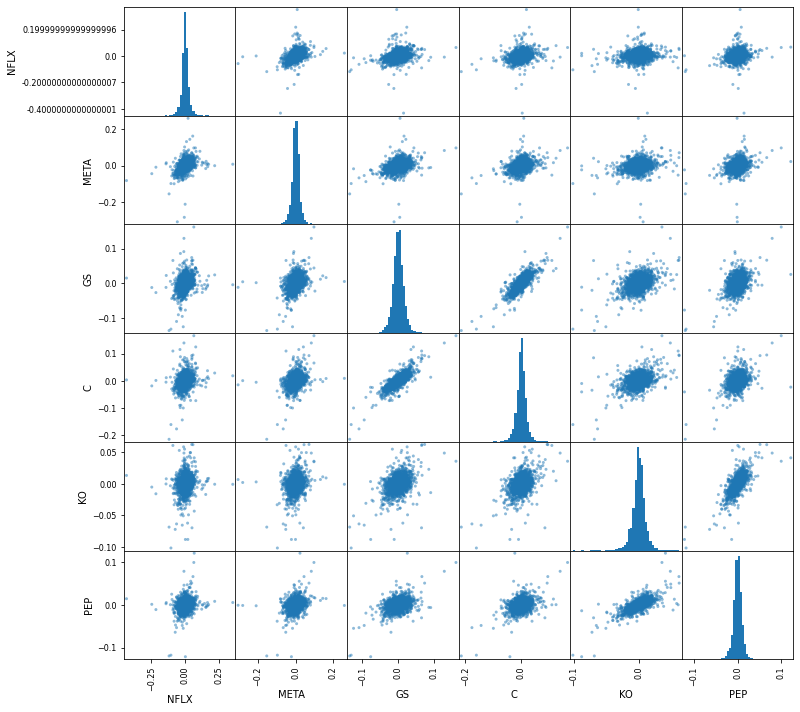
\includegraphics[width=0.5\textwidth, center]{scatterPlot.png}
[...]
\chapter{Analisi di previsione}
Per fare l'analisi di previsione ho deciso di usare una Support Vector Machine (SVM). Per prima cosa prendiamo i dati e li raggruppiamo mensilmente con il seguente codice:
\begin{lstlisting}[language=python]
    NFLXm = NFLX.groupby(pd.Grouper(freq='M')).last()
    METAm = META.groupby(pd.Grouper(freq='M')).last()
    GSm = GS.groupby(pd.Grouper(freq='M')).last()
    Cm = C.groupby(pd.Grouper(freq='M')).last()
    KOm = KO.groupby(pd.Grouper(freq='M')).last()
    PEPm = PEP.groupby(pd.Grouper(freq='M')).last()
\end{lstlisting}
Adesso possiamo procedere alla creazione delle "prediction". Quello che vogliamo ottenere è la predizione del prossimo mese di conseguenza la riga "prediction" è lo shift dei prezzi di una unità.

\begin{lstlisting}[language=python]
    df = GSm[['Adj Close']]
    forecast_out = 1
    monthPrevision = 10
    df['prediction'] = df[['Adj Close']].shift(-forecast_out)
    x = np.array(df.drop(['prediction'], 1))
    x = x[:-forecast_out]
    y = np.array(df['prediction'])
    y = y[:-forecast_out]
\end{lstlisting}

Ora andiamo avanti dividendo il nostro dataset in due, uno di allenamento e uno di test. In particolare le dimesioni dei due dataset sono 80 e 30 rispettivamente. Poi alleniamo la nostra SVM con il metodo \lstinline{.fit()} e otteniamo un primo valore che è quello di confidenza che è pari a \num{0.5844}

\begin{lstlisting}[language=python]
    #usiamo 30 mesi per il test e 80 per il train
    x_train, x_test, y_train, y_test = train_test_split(x, y, test_size=30, train_size=80)
    svr_rbf = SVR(kernel='rbf', C=1e3, gamma=0.1)
    svr_rbf.fit(x_train, y_train)
    svm_confidence = svr_rbf.score(x_test, y_test)
    print("svm confidence: ", round(svm_confidence, 4))
\end{lstlisting}

Prendiamo gli ultimi 10 mesi dei nostri prezzi per confrontare le previsioni rispetto ai valori effettivi e mostriamoli a grafico

\begin{lstlisting}[language=python]
    #prendiamo gli ultimi 10 mesi per fare la previsione
    x_mesi = np.array(df.drop(['prediction'], 1))[-monthPrevision:]
    y_mesi = np.array(df.drop(['Adj Close'], 1))[-monthPrevision:]
    
    #effettuiamo la previsione
    svm_prediction = svr_rbf.predict(x_mesi)
    plt.figure(figsize=(40,15))
    plt.plot(y_mesi, color='red', label='Real GS Stock Price')
    plt.plot(svm_prediction, color='blue', label='Predicted GS Stock Price')
    plt.title('GS Stock Price Prediction')
    plt.xlabel('Time')
    plt.ylabel('GS Stock Price')
    plt.legend()
    plt.show()
\end{lstlisting}
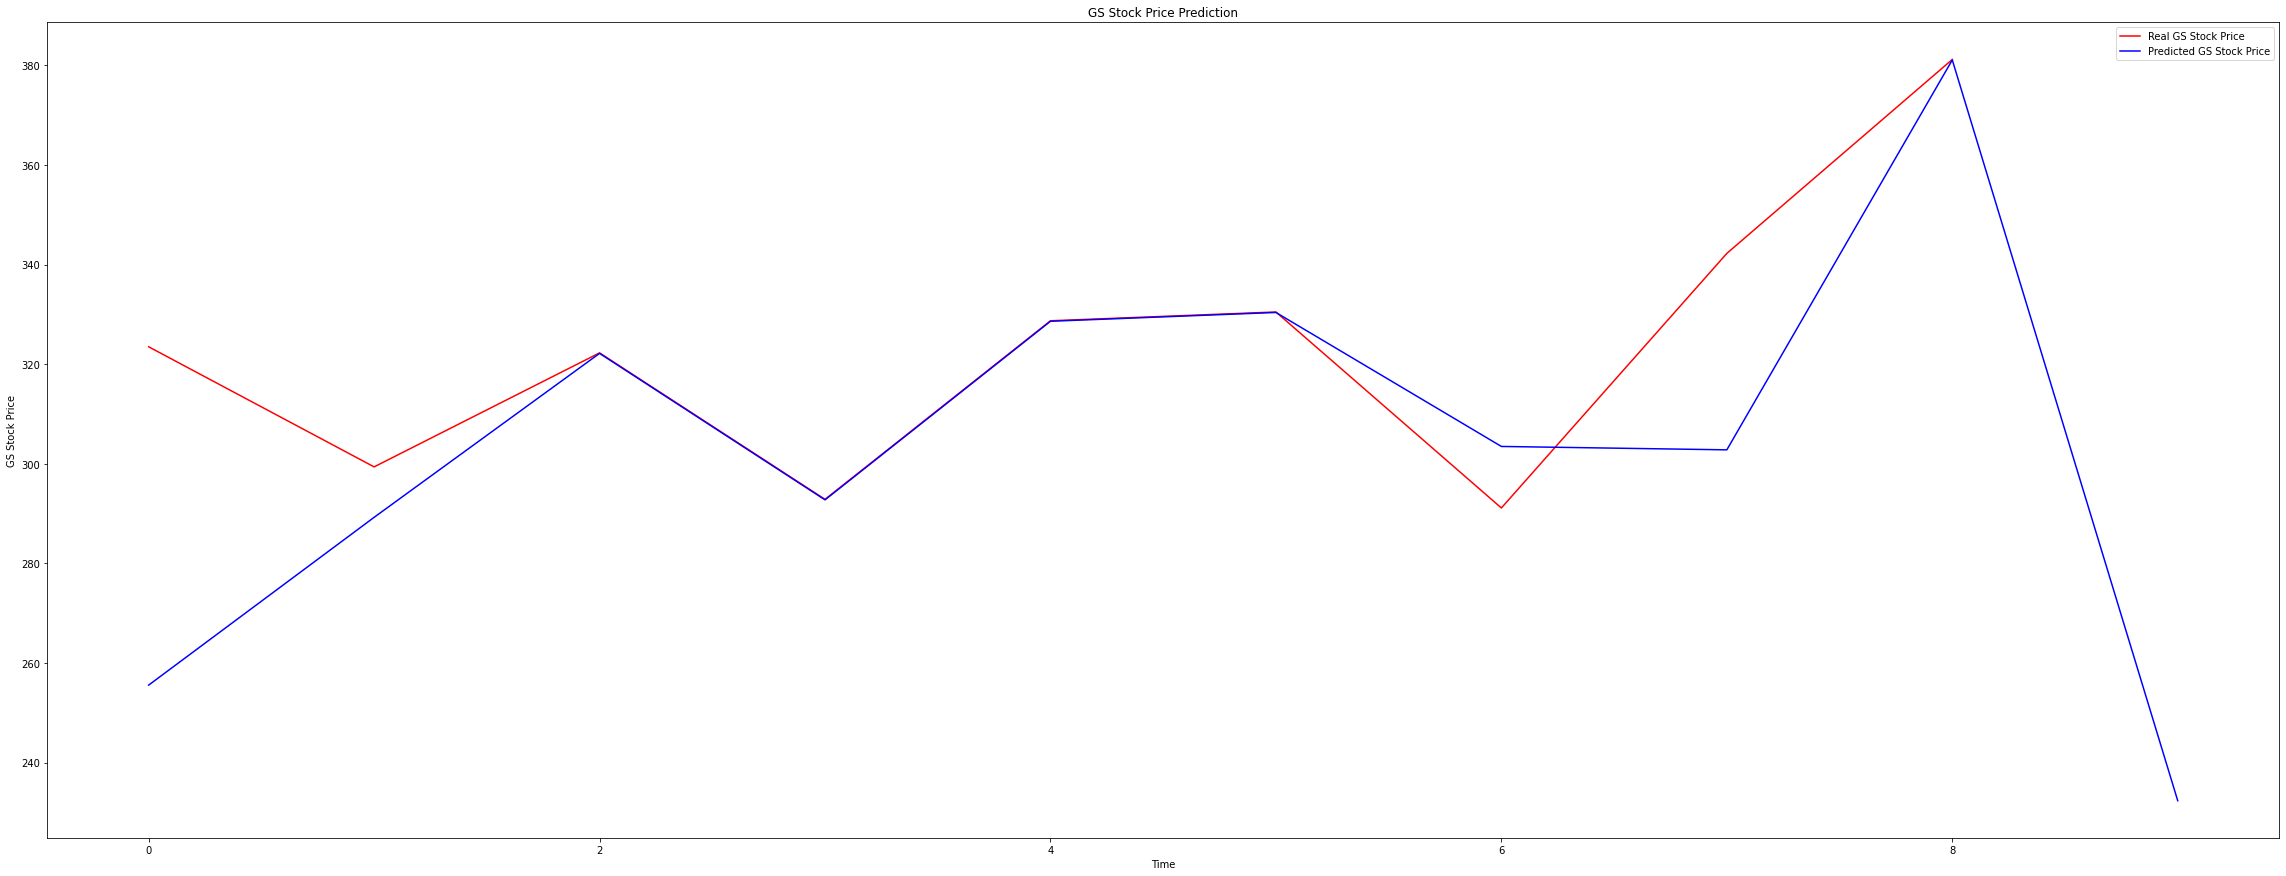
\includegraphics[width=0.6\textwidth, center]{svm.png}

\chapter{Strategia di trading e backtesting}
Come strategia di trading ho deciso di adottare l'indicatore \textbf{MACD} il cui acronimo sta per \textbf{Moving Average Convergence Divergence} che é un trend-following momentum indicator. Per calcolare questo indicatore sono necessarie tre Medie Mobili Esponenziali (\textbf{EMA}). La prima media mobile, quella più veloce, viene calcolata a 12 periodi; quella più lenta invece è a 26 periodi. Queste due medie mobili vengono sottratte fra loro per calcolarne la differenza che sarà quindi rappresentata graficamente da una sola linea (MACD Line). Per generare segnali è stata introdotta la terza linea, ovvero una media mobile esponenziale, solitamente a 9 periodi, della precedente differenza (Signal Line). Per generare un segnale di acquisto lungo, la MACD Line deve incrociare al rialzo la Signal Line.

Confronteremo la seguente strategia con una strategia Buy-and-Hold e con un strategia di incrocio di due Medie Mobili Semplici (\textbf{SMA}) sul prezzo. 
\section{Costruzione della strategia}
Quindi per prima cosa calcoliamo gli indicatori
\begin{lstlisting}[language=python]
    data = NFLX.drop(columns=['Open', 'High', 'Low',])
    data['SMA20'] = data['Adj Close'].rolling(20).mean()
    data['SMA120'] = data['Adj Close'].rolling(120).mean()
    exp1 = data['Close'].ewm(span=12, adjust = False).mean()
    exp2 = data['Close'].ewm(span=26, adjust = False).mean()
    data['MACD'] = exp1 - exp2
    data['Signal line'] = data['MACD'].ewm(span=9, adjust = False).mean()
    data.dropna()
\end{lstlisting}
Poi procediamo al calcolo dei segnali di acquisto e dei rendimenti delle strategia SMA e MACD
\begin{lstlisting}
    data['Price_yesterday'] = data['Adj Close'].shift(1)
    data['Change'] = data['Adj Close'] / data['Price_yesterday']
    
    #segnale aquisto strategia SMA
    data['Invested_SMA'] = [1 if data.loc[i, 'SMA20'] > data.loc[i, 'SMA120'] 
                            else 0 for i in data.index]
    
    #segnale acquisto strategia MACD
    data['Invested_MACD'] = [1 if data.loc[i, 'MACD'] > data.loc[i, 'Signal line']
                            else 0 for i in data.index]
    data = data.dropna()
    
    #calcolo strategia SMA
    sma = data[data['Invested_SMA'] == 1]
    sma['Return'] = np.cumprod(sma['Change'])
    sma['rtn'] =sma['Return'].pct_change()
    sma['rtn'].std()*np.sqrt(252)
    sma['rtn'].mean()*252 / (sma['rtn'].std()*np.sqrt(252))
    
    #calcolo strategia MACD
    macd = data[data['Invested_MACD'] == 1]
    macd['Return'] = np.cumprod(macd['Change'])
    macd['rtn'] =macd['Return'].pct_change()
    macd['rtn'].std()*np.sqrt(252)
    macd['rtn'].mean()*252 / (macd['rtn'].std()*np.sqrt(252))
\end{lstlisting}
\section{Misurazione efficienza della strategia}
Ora calcoliamo il rendimento di una strategia Buy-and-Hold con il seguente codice
\begin{lstlisting}[language=python]
    data['Buy_and_hold'] = np.cumprod(data['Change'])
    data['rtn'] = data['Buy_and_hold'].pct_change()
    data['rtn'].std()
    data['rtn'].mean()*252 / (data['rtn'].std()*np.sqrt(252))
\end{lstlisting}
Mostriamo graficamente ora i dati con il seguente codice in 4 diversi grafici:
\begin{lstlisting}
    plt.figure(figsize=(20,24))
    ax1 = plt.subplot2grid((12,1), (0,0), rowspan = 4, colspan = 1, title = 'NFLX')
    ax2 = plt.subplot2grid((12,1), (4,0), rowspan = 2, colspan = 1, sharex = ax1)
    ax3 = plt.subplot2grid((12,1), (6,0), rowspan = 2, colspan = 1, sharex = ax1)
    ax4 = plt.subplot2grid((12,1), (8,0), rowspan = 2, colspan = 1, sharex = ax1)
    
    ax1.plot(data['Adj Close'], label = 'Price')
    ax1.plot(data['SMA20'], label = 'SMA20')
    ax1.plot(data['SMA120'], label = 'SMA120')
    
    ax2.bar(data.index, data['Volume'], label = 'Volume')
    
    ax3.plot(data['MACD'], label = 'MACD')
    ax3.plot(data['Signal line'], label = 'Signal line')
    
    ax4.plot(data['Buy_and_hold'], label = 'Buy and hold')
    ax4.plot(sma['Return'], label = 'SMA')
    ax4.plot(macd['Return'], label = 'MACD')
    plt.gca().xaxis.set_major_formatter(mdates.DateFormatter('%Y-%m'))
    ax4.set_xlabel('Date (Year - month)')
    
    ax1.legend()
    ax2.legend()
    ax4.legend()
    ax3.legend()
    plt.show()
\end{lstlisting}

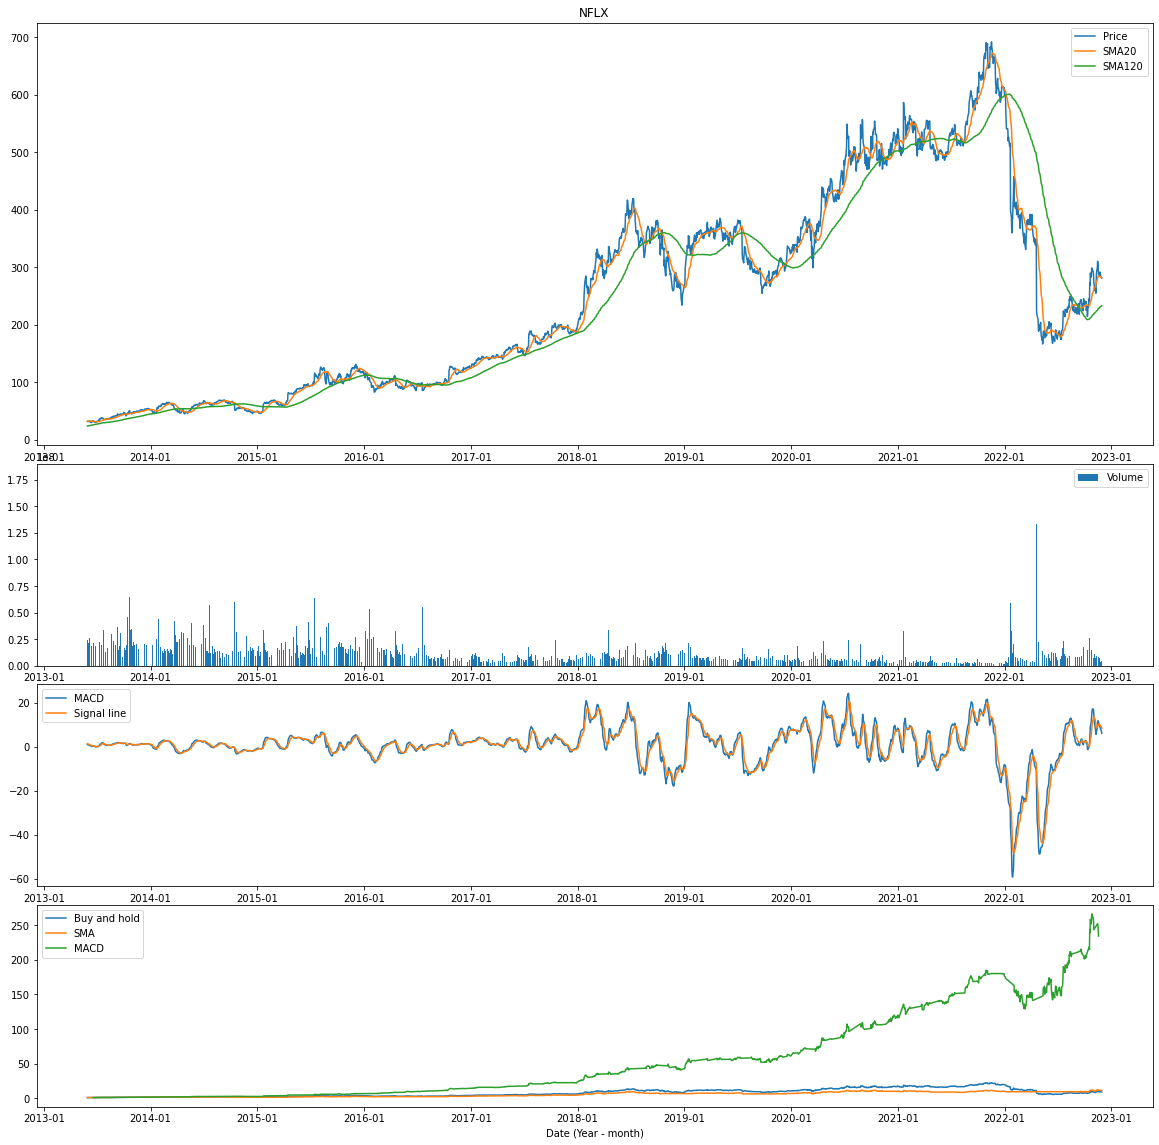
\includegraphics[width=1\textwidth, center]{MACD.png}

\chapter{Capital Asset Pricing Model}
Per prima cosa scarichiamo i dati dell'indice S&P 500 insieme ai titoli scelti in precedenza e sistemiamo il DataFrame
\begin{lstlisting}
    marketBenchmark = '^GSPC'
    df = yf.download(['NFLX', 'META', 'GS', 'C', 'KO', 'PEP', marketBenchmark], start, end)
    marketCloses = df['Adj Close']
    x = marketCloses.pct_change().dropna()
\end{lstlisting}
\section{Calcolo dei Beta rispetto al mercato}
Ora possiamo procedere al calcolo del Beta di ciascun titolo rispetto al mercato. Il seguente codice mostra il metodo utilizzato per Netflix, analogamente lo si puó usare per gli altri titoli:
\begin{lstlisting}
    #NFLX and S&P500 Beta
    NFLXMarket = pd.concat([x['NFLX'], x['^GSPC']], axis=1)
    covNFLX = NFLXMarket.cov().iloc[0,1]
    marketVariance = x['^GSPC'].var()
    betaNFLX = covNFLX/marketVariance
\end{lstlisting}
Ottenendo i seguenti valori: 

\begin{tabular}{lrrrrrr}
\toprule
{} &     NFLX &     META &      GS &        C &       KO &      PEP \\
\midrule
Beta &  1.154346 &  1.234385 &  1.204651 &  1.348596 &  0.633521 &  0.674546 \\

\bottomrule
\end{tabular}

\section{Fattori di rischio Fama French}

I tre fattori del modello di Fama e French (*) sono:
\begin{itemize}[leftmargin=30pt, rightmargin=2cm]
\item il fattore mercato, cioè la dipendenza dall'andamento del mercato azionario (\textbf{MKT})
\item il fattore dimensione (\textbf{SMB}) costruito come rendimento in eccesso delle azioni a piccola capitalizzazione rispetto alle grandi
\item il fattore valore (\textbf{HML}) costruito come rendimento in eccesso delle azioni con un rapporto fra patrimonio e prezzo alto (Value stocks) e quelle con un rapporto fra patriomonio e prezzo basso (Growth stocks)
\end{itemize}
Come prima cosa, per poter scaricare i dati del fattore Fama French importiamo la libreria \lstinline{pandas_datareader} nel seguente modo
\begin{lstlisting}
    import pandas_datareader as pdr
\end{lstlisting}
Poi procediamo con il download dei dati con la seguente funzione
\begin{lstlisting}
    factor_df = pdr.famafrench.FamaFrenchReader('F-F_Research_Data_Factors', start, end).read()[0]
\end{lstlisting}

I valori \lstinline{start} e \lstinline{end} sono i valori di inizio e fine del nostro periodo di analisi. Il nostro DataFrame \lstinline{factor_df} si presenta nel seguente modo:

\begin{tabular}{lrrrr}
\toprule
{} &     mkt &     smb &     hml &      rf \\
Date    &         &         &         &         \\
\midrule
2012-11 &  0.0078 &  0.0064 & -0.0084 &  0.0001 \\
2012-12 &  0.0118 &  0.0150 &  0.0351 &  0.0001 \\
2013-01 &  0.0557 &  0.0033 &  0.0096 &  0.0000 \\
2013-02 &  0.0129 & -0.0028 &  0.0011 &  0.0000 \\
2013-03 &  0.0403 &  0.0081 & -0.0019 &  0.0000 \\
\bottomrule
\end{tabular}

\subsection{NFLX Fama-French}
Procediamo poi al calcolo della regressione per i valori di Netflix con il seguente codice:

\begin{lstlisting}[language=python]
    #NFLX Fama French risk exposure
    y = NFLXm['Adj Close'].pct_change().dropna()
    
    #sistemiamo i mesi, per farli combaciare
    factor_df = factor_df.tail(-1)
    y = y.head(-1)
    
    #sistemiamo le date allo stesso formato
    y.index = y.index.strftime('%Y-%m')
    factor_df.index = factor_df.index.strftime('%Y-%m')
    
    #rinominiamo la colonna
    y.name = 'rtn'
    
    #uniamo i due dataframe
    ff_data = factor_df.join(y)
    
    #calcoliamo l'Excess Return
    ff_data['excess_rtn'] = ff_data.rtn - ff_data.rf
    
    #effettuiamo la regressione
    ff_model = smf.ols(formula = 'excess_rtn ~ mkt + smb + hml', data = ff_data).fit()
\end{lstlisting}
Il soprastante codice produce il seguente output:

\begin{center}
\begin{tabular}{lclc}
\toprule
\textbf{Dep. Variable:}    &   excess\_rtn    & \textbf{  R-squared:         } &     0.216   \\
\textbf{Model:}            &       OLS        & \textbf{  Adj. R-squared:    } &     0.195   \\
\textbf{Method:}           &  Least Squares   & \textbf{  F-statistic:       } &     10.54   \\
\textbf{Date:}             & Tue, 27 Dec 2022 & \textbf{  Prob (F-statistic):} &  3.53e-06   \\
\textbf{Time:}             &     14:53:46     & \textbf{  Log-Likelihood:    } &    77.670   \\
\textbf{No. Observations:} &         119      & \textbf{  AIC:               } &    -147.3   \\
\textbf{Df Residuals:}     &         115      & \textbf{  BIC:               } &    -136.2   \\
\textbf{Df Model:}         &           3      & \textbf{                     } &             \\
\bottomrule
\end{tabular}
\begin{tabular}{lcccccc}
                   & \textbf{coef} & \textbf{std err} & \textbf{t} & \textbf{P$> |$t$|$} & \textbf{[0.025} & \textbf{0.975]}  \\
\midrule
\textbf{Intercept} &       0.0221  &        0.012     &     1.824  &         0.071        &       -0.002    &        0.046     \\
\textbf{mkt}       &       1.3657  &        0.281     &     4.858  &         0.000        &        0.809    &        1.923     \\
\textbf{smb}       &      -0.0198  &        0.483     &    -0.041  &         0.967        &       -0.977    &        0.937     \\
\textbf{hml}       &      -0.8983  &        0.334     &    -2.693  &         0.008        &       -1.559    &       -0.238     \\
\bottomrule
\end{tabular}
\begin{tabular}{lclc}
\textbf{Omnibus:}       & 59.945 & \textbf{  Durbin-Watson:     } &    1.717  \\
\textbf{Prob(Omnibus):} &  0.000 & \textbf{  Jarque-Bera (JB):  } &  296.596  \\
\textbf{Skew:}          &  1.655 & \textbf{  Prob(JB):          } & 3.94e-65  \\
\textbf{Kurtosis:}      &  9.991 & \textbf{  Cond. No.          } &     42.0  \\
\bottomrule
\end{tabular}
%\caption{OLS Regression Results}
\end{center}

Analogamente calcoliamo l'esposizione di ogni titolo ai fattori di rischio

\subsection{META Fama-French}
\begin{center}
\begin{tabular}{lclc}
\toprule
\textbf{Dep. Variable:}    &   excess\_rtn    & \textbf{  R-squared:         } &     0.243   \\
\textbf{Model:}            &       OLS        & \textbf{  Adj. R-squared:    } &     0.223   \\
\textbf{Method:}           &  Least Squares   & \textbf{  F-statistic:       } &     12.30   \\
\textbf{Date:}             & Tue, 27 Dec 2022 & \textbf{  Prob (F-statistic):} &  4.90e-07   \\
\textbf{Time:}             &     15:04:42     & \textbf{  Log-Likelihood:    } &    120.19   \\
\textbf{No. Observations:} &         119      & \textbf{  AIC:               } &    -232.4   \\
\textbf{Df Residuals:}     &         115      & \textbf{  BIC:               } &    -221.3   \\
\textbf{Df Model:}         &           3      & \textbf{                     } &             \\
\bottomrule
\end{tabular}
\begin{tabular}{lcccccc}
                   & \textbf{coef} & \textbf{std err} & \textbf{t} & \textbf{P$> |$t$|$} & \textbf{[0.025} & \textbf{0.975]}  \\
\midrule
\textbf{Intercept} &       0.0029  &        0.008     &     0.348  &         0.729        &       -0.014    &        0.020     \\
\textbf{mkt}       &       1.1127  &        0.197     &     5.658  &         0.000        &        0.723    &        1.502     \\
\textbf{smb}       &      -0.3803  &        0.338     &    -1.125  &         0.263        &       -1.050    &        0.289     \\
\textbf{hml}       &      -0.5585  &        0.233     &    -2.394  &         0.018        &       -1.021    &       -0.096     \\
\bottomrule
\end{tabular}
\begin{tabular}{lclc}
\textbf{Omnibus:}       & 24.295 & \textbf{  Durbin-Watson:     } &    1.707  \\
\textbf{Prob(Omnibus):} &  0.000 & \textbf{  Jarque-Bera (JB):  } &  166.493  \\
\textbf{Skew:}          &  0.216 & \textbf{  Prob(JB):          } & 7.02e-37  \\
\textbf{Kurtosis:}      &  8.779 & \textbf{  Cond. No.          } &     42.0  \\
\bottomrule
\end{tabular}
%\caption{OLS Regression Results}

\end{center}
\subsection{GS Fama-French}

\begin{center}
\begin{tabular}{lclc}
\toprule
\textbf{Dep. Variable:}    &   excess\_rtn    & \textbf{  R-squared:         } &     0.676   \\
\textbf{Model:}            &       OLS        & \textbf{  Adj. R-squared:    } &     0.667   \\
\textbf{Method:}           &  Least Squares   & \textbf{  F-statistic:       } &     79.93   \\
\textbf{Date:}             & Tue, 27 Dec 2022 & \textbf{  Prob (F-statistic):} &  5.23e-28   \\
\textbf{Time:}             &     15:17:45     & \textbf{  Log-Likelihood:    } &    199.72   \\
\textbf{No. Observations:} &         119      & \textbf{  AIC:               } &    -391.4   \\
\textbf{Df Residuals:}     &         115      & \textbf{  BIC:               } &    -380.3   \\
\textbf{Df Model:}         &           3      & \textbf{                     } &             \\
\bottomrule
\end{tabular}
\begin{tabular}{lcccccc}
                   & \textbf{coef} & \textbf{std err} & \textbf{t} & \textbf{P$> |$t$|$} & \textbf{[0.025} & \textbf{0.975]}  \\
\midrule
\textbf{Intercept} &      -0.0006  &        0.004     &    -0.127  &         0.899        &       -0.009    &        0.008     \\
\textbf{mkt}       &       1.3185  &        0.101     &    13.081  &         0.000        &        1.119    &        1.518     \\
\textbf{smb}       &       0.2460  &        0.173     &     1.419  &         0.158        &       -0.097    &        0.589     \\
\textbf{hml}       &       0.6648  &        0.120     &     5.559  &         0.000        &        0.428    &        0.902     \\
\bottomrule
\end{tabular}
\begin{tabular}{lclc}
\textbf{Omnibus:}       &  3.869 & \textbf{  Durbin-Watson:     } &    2.068  \\
\textbf{Prob(Omnibus):} &  0.144 & \textbf{  Jarque-Bera (JB):  } &    4.502  \\
\textbf{Skew:}          & -0.091 & \textbf{  Prob(JB):          } &    0.105  \\
\textbf{Kurtosis:}      &  3.935 & \textbf{  Cond. No.          } &     42.0  \\
\bottomrule
\end{tabular}
%\caption{OLS Regression Results}
\end{center}

\subsection{C Fama-French}

\begin{center}
\begin{tabular}{lclc}
\toprule
\textbf{Dep. Variable:}    &   excess\_rtn    & \textbf{  R-squared:         } &     0.724   \\
\textbf{Model:}            &       OLS        & \textbf{  Adj. R-squared:    } &     0.717   \\
\textbf{Method:}           &  Least Squares   & \textbf{  F-statistic:       } &     100.5   \\
\textbf{Date:}             & Tue, 27 Dec 2022 & \textbf{  Prob (F-statistic):} &  5.32e-32   \\
\textbf{Time:}             &     15:19:03     & \textbf{  Log-Likelihood:    } &    194.52   \\
\textbf{No. Observations:} &         119      & \textbf{  AIC:               } &    -381.0   \\
\textbf{Df Residuals:}     &         115      & \textbf{  BIC:               } &    -369.9   \\
\textbf{Df Model:}         &           3      & \textbf{                     } &             \\
\bottomrule
\end{tabular}
\begin{tabular}{lcccccc}
                   & \textbf{coef} & \textbf{std err} & \textbf{t} & \textbf{P$> |$t$|$} & \textbf{[0.025} & \textbf{0.975]}  \\
\midrule
\textbf{Intercept} &      -0.0077  &        0.005     &    -1.692  &         0.093        &       -0.017    &        0.001     \\
\textbf{mkt}       &       1.4752  &        0.105     &    14.010  &         0.000        &        1.267    &        1.684     \\
\textbf{smb}       &       0.1708  &        0.181     &     0.944  &         0.347        &       -0.188    &        0.529     \\
\textbf{hml}       &       1.0114  &        0.125     &     8.096  &         0.000        &        0.764    &        1.259     \\
\bottomrule
\end{tabular}
\begin{tabular}{lclc}
\textbf{Omnibus:}       &  0.264 & \textbf{  Durbin-Watson:     } &    1.837  \\
\textbf{Prob(Omnibus):} &  0.876 & \textbf{  Jarque-Bera (JB):  } &    0.121  \\
\textbf{Skew:}          & -0.077 & \textbf{  Prob(JB):          } &    0.942  \\
\textbf{Kurtosis:}      &  3.029 & \textbf{  Cond. No.          } &     42.0  \\
\bottomrule
\end{tabular}
%\caption{OLS Regression Results}
\end{center}

\subsection{KO Fama-French}

\begin{center}
\begin{tabular}{lclc}
\toprule
\textbf{Dep. Variable:}    &   excess\_rtn    & \textbf{  R-squared:         } &     0.434   \\
\textbf{Model:}            &       OLS        & \textbf{  Adj. R-squared:    } &     0.419   \\
\textbf{Method:}           &  Least Squares   & \textbf{  F-statistic:       } &     29.37   \\
\textbf{Date:}             & Tue, 27 Dec 2022 & \textbf{  Prob (F-statistic):} &  3.57e-14   \\
\textbf{Time:}             &     15:20:01     & \textbf{  Log-Likelihood:    } &    231.66   \\
\textbf{No. Observations:} &         119      & \textbf{  AIC:               } &    -455.3   \\
\textbf{Df Residuals:}     &         115      & \textbf{  BIC:               } &    -444.2   \\
\textbf{Df Model:}         &           3      & \textbf{                     } &             \\
\bottomrule
\end{tabular}
\begin{tabular}{lcccccc}
                   & \textbf{coef} & \textbf{std err} & \textbf{t} & \textbf{P$> |$t$|$} & \textbf{[0.025} & \textbf{0.975]}  \\
\midrule
\textbf{Intercept} &       0.0002  &        0.003     &     0.057  &         0.955        &       -0.006    &        0.007     \\
\textbf{mkt}       &       0.6516  &        0.077     &     8.455  &         0.000        &        0.499    &        0.804     \\
\textbf{smb}       &      -0.7616  &        0.132     &    -5.749  &         0.000        &       -1.024    &       -0.499     \\
\textbf{hml}       &       0.1742  &        0.091     &     1.905  &         0.059        &       -0.007    &        0.355     \\
\bottomrule
\end{tabular}
\begin{tabular}{lclc}
\textbf{Omnibus:}       &  0.634 & \textbf{  Durbin-Watson:     } &    2.422  \\
\textbf{Prob(Omnibus):} &  0.728 & \textbf{  Jarque-Bera (JB):  } &    0.289  \\
\textbf{Skew:}          & -0.078 & \textbf{  Prob(JB):          } &    0.866  \\
\textbf{Kurtosis:}      &  3.185 & \textbf{  Cond. No.          } &     42.0  \\
\bottomrule
\end{tabular}
%\caption{OLS Regression Results}
\end{center}

\subsection{PEP Fama-French}

\begin{center}
\begin{tabular}{lclc}
\toprule
\textbf{Dep. Variable:}    &   excess\_rtn    & \textbf{  R-squared:         } &     0.441   \\
\textbf{Model:}            &       OLS        & \textbf{  Adj. R-squared:    } &     0.427   \\
\textbf{Method:}           &  Least Squares   & \textbf{  F-statistic:       } &     30.27   \\
\textbf{Date:}             & Tue, 27 Dec 2022 & \textbf{  Prob (F-statistic):} &  1.69e-14   \\
\textbf{Time:}             &     15:20:51     & \textbf{  Log-Likelihood:    } &    243.18   \\
\textbf{No. Observations:} &         119      & \textbf{  AIC:               } &    -478.4   \\
\textbf{Df Residuals:}     &         115      & \textbf{  BIC:               } &    -467.2   \\
\textbf{Df Model:}         &           3      & \textbf{                     } &             \\
\bottomrule
\end{tabular}
\begin{tabular}{lcccccc}
                   & \textbf{coef} & \textbf{std err} & \textbf{t} & \textbf{P$> |$t$|$} & \textbf{[0.025} & \textbf{0.975]}  \\
\midrule
\textbf{Intercept} &       0.0041  &        0.003     &     1.365  &         0.175        &       -0.002    &        0.010     \\
\textbf{mkt}       &       0.6386  &        0.070     &     9.129  &         0.000        &        0.500    &        0.777     \\
\textbf{smb}       &      -0.6303  &        0.120     &    -5.240  &         0.000        &       -0.869    &       -0.392     \\
\textbf{hml}       &      -0.0088  &        0.083     &    -0.106  &         0.916        &       -0.173    &        0.156     \\
\bottomrule
\end{tabular}
\begin{tabular}{lclc}
\textbf{Omnibus:}       &  0.613 & \textbf{  Durbin-Watson:     } &    2.344  \\
\textbf{Prob(Omnibus):} &  0.736 & \textbf{  Jarque-Bera (JB):  } &    0.549  \\
\textbf{Skew:}          &  0.164 & \textbf{  Prob(JB):          } &    0.760  \\
\textbf{Kurtosis:}      &  2.944 & \textbf{  Cond. No.          } &     42.0  \\
\bottomrule
\end{tabular}
%\caption{OLS Regression Results}
\end{center}

Possiamo notare che in tutti e 6 i titoli il fattore di rischio maggiore é \textbf{mkt} che corrisponde al mercato

\section{Calcoliamo il rendimento atteso annuo}
Per calcolare i rendimenti attesi dobbiamo utilizzare i dati di Fama-French
\begin{lstlisting}
    risk_free = factor_df['rf'].mean()
    market_prem = factor_df['mkt'].mean()
\end{lstlisting}

\noindent\textbf{Risk Free Rate}:  0.0005433333333333336

\noindent\textbf{Market Premium}:  0.010717499999999998

Definiamo la seguente funzione per calcolare i rendimenti attesi tra un anno
\begin{lstlisting}
    def expectedReturn(beta):
        return (risk_free + beta*(market_prem - risk_free)) * 12
\end{lstlisting}
Usiamo i beta calcolati in precedenza per calcolare i valori
\begin{lstlisting}
    NFLXexpectedReturns = expectedReturn(betaNFLX)
    METAexpectedReturns = expectedReturn(betaMETA)
    GSexpectedReturns = expectedReturn(betaGS)
    CexpectedReturns = expectedReturn(betaC)
    KOexpectedReturns = expectedReturn(betaKO)
    PEPexpectedReturns = expectedReturn(betaPEP)
    expectedReturns = pd.DataFrame({'NFLX': NFLXexpectedReturns, 'META': METAexpectedReturns, 'GS': GSexpectedReturns, 'C': CexpectedReturns, 'KO': KOexpectedReturns, 'PEP': PEPexpectedReturns}, index = ['Expected Returns'])
\end{lstlisting}

\begin{tabular}{lrrrrrr}
\toprule
{} &      NFLX &      META &        GS &        C &        KO &       PEP \\
\midrule
Expected Returns &  0.147454 &  0.157226 &  0.153596 &  0.17117 &  0.083867 &  0.088875 \\
\bottomrule
\end{tabular}


\chapter{Creazione di un portafoglio}
\section{Simulazione del portafogli con metodo Monte Carlo}
Creiamo ora un portafoglio composto dalle nostre 6 azioni. Quindi per prima cosa prendiamo i dati e calcoliamo alcune formule:
\begin{lstlisting}[language=python]
    N_PORTFOLIOS = 10 ** 5
    N_DAYS = 252
    prices_df = yf.download(["NFLX","META", "GS", "C", "KO", "PEP"], start, end, adjusted=True)
    returns_df = prices_df['Adj Close'].pct_change().dropna()
    avg_returns = returns_df.mean() * N_DAYS
    cov_mat = returns_df.cov() * N_DAYS
\end{lstlisting}
Calcoliamo ora il ritorno annualizzato e la deviazione standard corrispondente.
\begin{lstlisting}[language=python]
    returns_df = prices_df['Adj Close'].pct_change().dropna()
    avg_returns = returns_df.mean() * N_DAYS
    cov_mat = returns_df.cov() * N_DAYS
\end{lstlisting}
Simuliamo dei portafogli randomici
\begin{lstlisting}[language=python]
    np.random.seed(42)
    weights = np.random.random(size=(N_PORTFOLIOS, 6))
    weights /= np.sum(weights, axis=1)[:, np.newaxis]
\end{lstlisting}
Calcoliamo le metriche di questi portafogli, ovvero:

\begin{itemize}[leftmargin=30pt, rightmargin=2cm]
\item Volatilitá
\item Sharpe ratio
\item Ritorni
\end{itemize}

\begin{lstlisting}[language=python]
    portf_rtns = np.dot(weights, avg_returns)
    portf_vol = []
    for i in range(0, len(weights)):
        portf_vol.append(np.sqrt(np.dot(weights[i].T, np.dot(cov_mat, weights[i]))))
    portf_vol = np.array(portf_vol)
    portf_sharpe_ratio = portf_rtns / portf_vol
\end{lstlisting}
Ora che abbiamo tutti i dati, localizziamo i portafogli e creiamo la frontiera efficiente
\begin{lstlisting}[language=python]
    portf_results_df = pd.DataFrame({'returns': portf_rtns, 'volatility': portf_vol, 'sharpe_ratio': portf_sharpe_ratio})
    N_POINTS = 100
    portf_vol_ef = []
    indices_to_skip = []
    portf_rtns_ef = np.linspace(portf_results_df.returns.min(), portf_results_df.returns.max(), N_POINTS)
    portf_rtns_ef = np.round(portf_rtns_ef, 2)
    portf_rtns = np.round(portf_rtns, 2)
    for point_index in range(N_POINTS):
        if portf_rtns_ef[point_index] not in portf_rtns:
            indices_to_skip.append(point_index)
            continue
        matched_ind = np.where(portf_rtns == portf_rtns_ef[point_index])
        portf_vol_ef.append(np.min(portf_vol[matched_ind]))
    portf_rtns_ef = np.delete(portf_rtns_ef, indices_to_skip)
\end{lstlisting}
Ora, non ci resta che plottare la frontiera efficiente
\begin{lstlisting}[language=python]
    RISKY_ASSETS = ['NFLX', 'META', 'GS', 'C', 'KO', 'PEP']
    n_assets = len(RISKY_ASSETS)
    MARKS = ['o', 'X', 'd', '*', 'P', 'h']
    
    fig, ax = plt.subplots()
    fig.set_size_inches(20, 15)
    portf_results_df.plot(kind='scatter', x='volatility', y='returns', c='sharpe_ratio', cmap='RdYlGn', edgecolors='black', ax=ax)
    ax.set(xlabel='Volatility', ylabel='Expected Returns', title='Efficient Frontier')
    ax.plot(portf_vol_ef, portf_rtns_ef, 'b--')
    for asset_index in range(n_assets):
        ax.scatter(x=np.sqrt(cov_mat.iloc[asset_index, asset_index]), y=avg_returns[asset_index], marker=MARKS[asset_index], s=150, color='black', label=RISKY_ASSETS[asset_index])
    ax.legend()
\end{lstlisting}
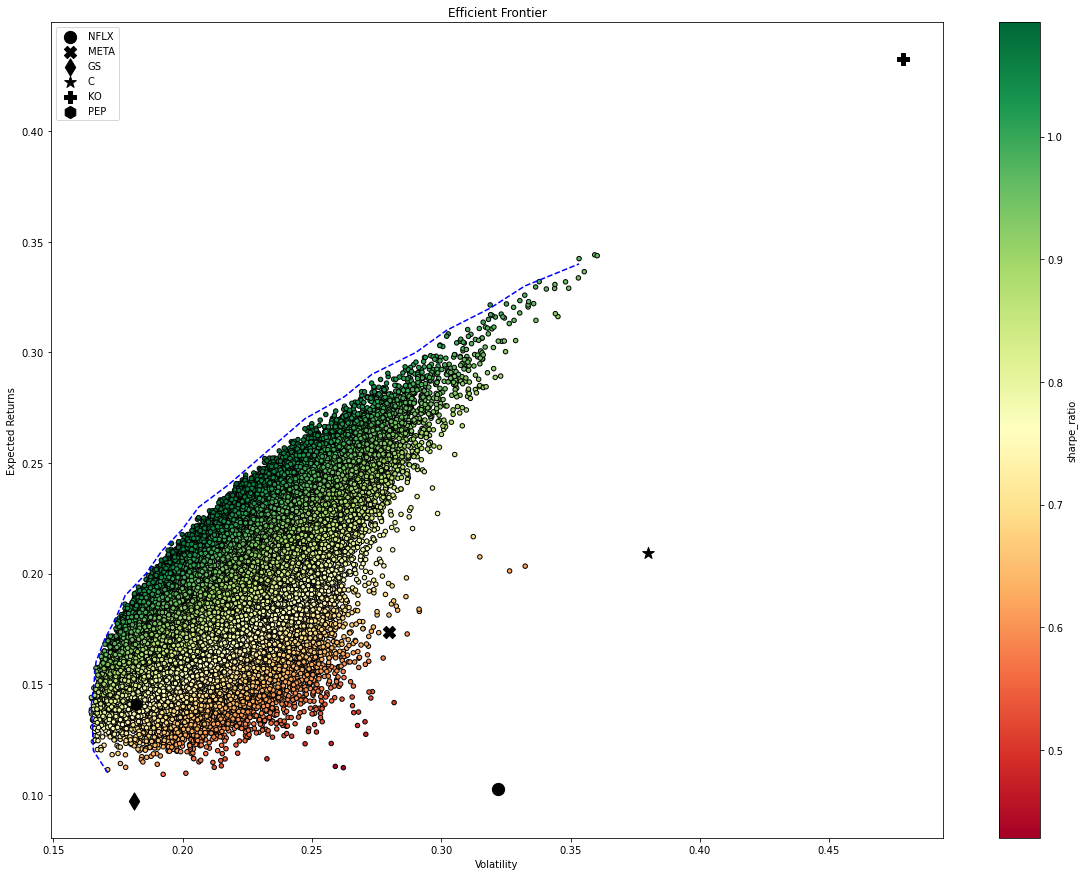
\includegraphics[width=1\textwidth, center]{frontieraEfficiente.png}
Ora possiamo trovare due portafogli importanti, il primo é quello costituito per diminuire il piú possibile la volatilitá, il secondo per massimizzare lo sharpe ratio, e sono i seguenti:
\begin{lstlisting}[]
    Minimum Volatility portfolio ----
    Performance
    returns: 13.75% volatility: 16.46% sharpe_ratio: 83.54% 
    Weights
    NFLX: 2.28% META: 2.40% GS: 44.51% C: 3.89% KO: 4.54% PEP: 42.38%
\end{lstlisting}

\begin{lstlisting}
    Maximum Sharpe ratio portfolio ----
    Performance
    returns: 22.53% volatility: 20.61% sharpe_ratio: 109.30% 
    Weights
    NFLX: 0.61% META: 15.44% GS: 7.14% C: 5.23% KO: 27.08% PEP: 44.50% 
\end{lstlisting}
\section{Creazione di portafogli con metodo analitico}
\subsection{Rendimenti passati}
Procediamo ora con la costruzione di un portafogli con metodo analitico.
Per prima cosa scarichiamo i dati mensili dei nostri titoli e dello strumento risk free SPY:
\begin{lstlisting}[language=python]
    tickers = ['NFLX', 'META', 'GS', 'C', 'KO', 'PEP', 'SPY']
    data = yf.download(tickers, start, end, interval='1mo')
\end{lstlisting}
Quindi prendiamo i primi 108 mesi e costruiamo un portafoglio basato sui rendimenti passti. In particolare usando le matrici di covarianza e di correlazione
\begin{lstlisting}[language=python]
    data = data[:108]
    returns = data['Adj Close'].pct_change().dropna()
    
    number_of_portfolios = 40000
    
    rf = returns['SPY'].mean() * 12
    returns.drop('SPY', axis = 1, inplace = True)
    means = returns.mean() * 12
    
    mat_cov = returns.cov()*12
    
    mat_corr = returns.corr()
    
    
    portfolio_returns = []
    portfolio_risks = []
    sharpe_ratios = []
    portfolio_weights = []
    
    for portfolio in range(number_of_portfolios):
        weights = np.random.random_sample(len(returns.columns))
        weights =np.round((weights / np.sum(weights)), 3)
        portfolio_weights.append(weights)
        annualized_return = np.sum(means * weights)
        portfolio_returns.append(annualized_return)
        portfolio_variance = np.dot(weights.T, np.dot(mat_cov, weights))
        portfolio_standard_deviation = np.sqrt(portfolio_variance)
        portfolio_risks.append(portfolio_standard_deviation)
        sharpe_ratio = (annualized_return - rf) / portfolio_standard_deviation
        sharpe_ratios.append(sharpe_ratio)
    
    
    portfolio_returns = np.array(portfolio_returns)
    portofolio_risks = np.array(portfolio_risks)
    sharpe_ratios = np.array(sharpe_ratios)
    
    portfolio_metrics = [portfolio_returns, portfolio_risks, sharpe_ratios, portfolio_weights]
    portfolios_df = pd.DataFrame(portfolio_metrics).T
    portfolios_df.columns = ['Return', 'Risk', 'Sharpe', 'Weights']
    
    min_risk = portfolios_df.iloc[portfolios_df['Risk'].astype(float).idxmin()]
    highest_return = portfolios_df.iloc[portfolios_df['Return'].astype(float).idxmax()]
    highest_sharpe = portfolios_df.iloc[portfolios_df['Sharpe'].astype(float).idxmax()]
\end{lstlisting}
Per mostrare il risultato usiamo il seguente codice:
\begin{lstlisting}[language=python]
    plt.figure(figsize = (10,5))
    plt.scatter(portfolio_risks, portfolio_returns, 
               c = (portfolio_returns - rf)/ portfolio_risks)
    plt.title('Portfolio optimization - Past returns', fontsize = 20)
    plt.xlabel('Volatility', fontsize = 18)
    plt.ylabel('Return', fontsize = 18)
    plt.xticks(fontsize = 15)
    plt.yticks(fontsize = 15)
    plt.colorbar(label = 'Sharpe ratio')
    plt.show()
\end{lstlisting}

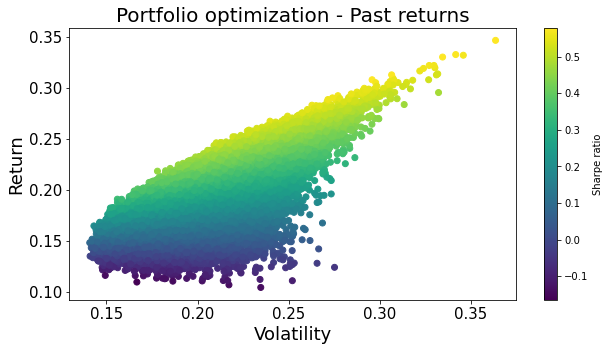
\includegraphics[width=1\textwidth, center]{portafogliPast.png}

Da questi dati otteniamo i seguenti risultati:

\textbf{Lowest risk}

\begin{tabular}{ll}
\toprule
{} &                                       20599 \\
\midrule
Return  &                                    0.148689 \\
Risk    &                                    0.136418 \\
Sharpe  &                                   -0.083582 \\
Weights &  [0.017, 0.083, 0.312, 0.086, 0.023, 0.478] \\
\bottomrule
\end{tabular}

\textbf{Highest return}

\begin{tabular}{ll}
\toprule
{} &                                      25629 \\
\midrule
Return  &                                   0.435404 \\
Risk    &                                   0.338331 \\
Sharpe  &                                   0.813738 \\
Weights &  [0.066, 0.005, 0.031, 0.209, 0.659, 0.03] \\
\bottomrule
\end{tabular}

\textbf{Highest Sharpe ratio}

\begin{tabular}{ll}
\toprule
{} &                                        1394 \\
\midrule
Return  &                                    0.420549 \\
Risk    &                                    0.315616 \\
Sharpe  &                                    0.825237 \\
Weights &  [0.009, 0.056, 0.022, 0.265, 0.586, 0.061] \\
\bottomrule
\end{tabular}

\subsection{Rendimenti attesi}

Analogamente prendiamo i valori calcolati nel punto 5 dei rendimenti attesi e usiamo per creare il portafogli:
\begin{lstlisting}[language=python]
    d = {'NFLX': NFLXexpectedReturns, 'META': METAexpectedReturns, 'GS': GSexpectedReturns, 'C': CexpectedReturns, 'KO': KOexpectedReturns, 'PEP': PEPexpectedReturns}
    means_exp = pd.Series(data=d, index=['NFLX', 'META', 'GS', 'C', 'KO', 'PEP'])
\end{lstlisting}
Procediamo come fatto in precedenza alla creazione del portafogli
\begin{lstlisting}[language=python]
    portfolio_returns = []
    portfolio_risks = []
    sharpe_ratios = []
    portfolio_weights = []
    rf_exp = 0.02
    target = 0.06
    
    for portfolio in range(number_of_portfolios):
        weights = np.random.random_sample(len(returns.columns))
        weights =np.round((weights / np.sum(weights)), 3)
        portfolio_weights.append(weights)
        annualized_return = np.sum(means_exp * weights)
        portfolio_returns.append(annualized_return)
        portfolio_variance = np.dot(weights.T, np.dot(mat_cov, weights))
        portfolio_standard_deviation = np.sqrt(portfolio_variance)
        portfolio_risks.append(portfolio_standard_deviation)
        sharpe_ratio = (annualized_return - rf_exp) / portfolio_standard_deviation
        sharpe_ratios.append(sharpe_ratio)
    
    portfolio_returns = np.array(portfolio_returns)
    portofolio_risks = np.array(portfolio_risks)
    sharpe_ratios = np.array(sharpe_ratios)
    
    
    portfolio_metrics = [portfolio_returns, portfolio_risks, sharpe_ratios, portfolio_weights]
    portfolios_df = pd.DataFrame(portfolio_metrics).T
    portfolios_df.columns = ['Return', 'Risk', 'Sharpe', 'Weights']
    
    min_risk = portfolios_df.iloc[portfolios_df['Risk'].astype(float).idxmin()]
    highest_return = portfolios_df.iloc[portfolios_df['Return'].astype(float).idxmax()]
    highest_sharpe = portfolios_df.iloc[portfolios_df['Sharpe'].astype(float).idxmax()]
\end{lstlisting}

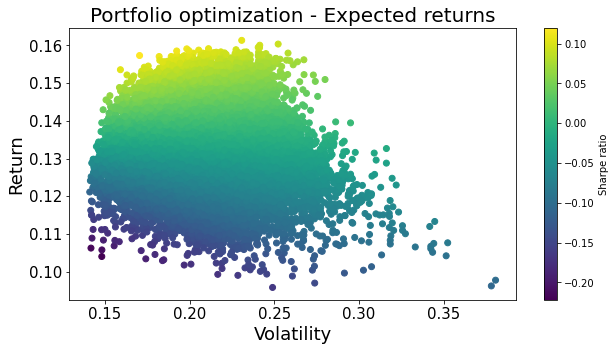
\includegraphics[width=1\textwidth, center]{portafogliExpect.png}

Con i seguenti risulati:

\textbf{Lowest risk}

\begin{tabular}{ll}
\toprule
{} &                                       20599 \\
\midrule
Return  &                                    0.148689 \\
Risk    &                                    0.136418 \\
Sharpe  &                                   -0.083582 \\
Weights &  [0.017, 0.083, 0.312, 0.086, 0.023, 0.478] \\
\bottomrule
\end{tabular}

\textbf{Highest return}

\begin{tabular}{ll}
\toprule
{} &                                      25629 \\
\midrule
Return  &                                   0.435404 \\
Risk    &                                   0.338331 \\
Sharpe  &                                   0.813738 \\
Weights &  [0.066, 0.005, 0.031, 0.209, 0.659, 0.03] \\
\bottomrule
\end{tabular}

\textbf{Highest Sharpe ratio}

\begin{tabular}{ll}
\toprule
{} &                                        1394 \\
\midrule
Return  &                                    0.420549 \\
Risk    &                                    0.315616 \\
Sharpe  &                                    0.825237 \\
Weights &  [0.009, 0.056, 0.022, 0.265, 0.586, 0.061] \\
\bottomrule
\end{tabular}


\section{Calcolo dei beta e dei rendimenti dei portafogli}

Ora invece procediamo con l'analisi delle performance dei portafogli che abbiamo costruito, in particolare confontandoli con il mercato e con un portafoglio costituito con i pesi equamente distribuiti, nel seguente modo:  \(\frac{1}{\text{number of assets}}\). Quindi per prima cosa riprendiamoci il valore del mercato scaricato in precedenza e calcoliamone i ritorni: \lstinline{benchmark = marketCloses['^GSPC'].pct_change().dropna()}. Ora tramite la libreria \lstinline{pyfolio} possiamo avere molti dati e grafici direttamente passando le serie, quindi procediamo con l'installazione e l'importo. (Da notare che la libreria originale é stata sostituita con la versione \lstinline{reloaded}, in quanto non piú supportata)
\begin{lstlisting}
    pip install pyfolio-reloaded
    import pyfolio as pf
\end{lstlisting}
Ora possiamo quindi procedere al calcolo delle serie e produrre il \lstinline{tear_sheet} e i dati con il seguente codice:
\begin{lstlisting}[language=python]
    portfolio_weights = n_assets * [1 / n_assets]
    portfolio_returns = pd.Series(np.dot(portfolio_weights, returns_df.T),
                                              index=returns_df.index)
    pf.create_returns_tear_sheet(portfolio_returns, benchmark_rets=benchmark)
\end{lstlisting}
 Analogamente eseguiamo lo stesso comando con i pesi calcolati in precedenza
 e otteniamo i seguenti valori di beta:

\begin{tabular}{lrrr}
\toprule
{} &     1/n &     Sharpe &      Volatility \\
\midrule
Beta &  1.04 &  0.92 &  0.73 \\

\bottomrule
\end{tabular}

\begin{figure}[h]

\begin{subfigure}{0.5\textwidth}
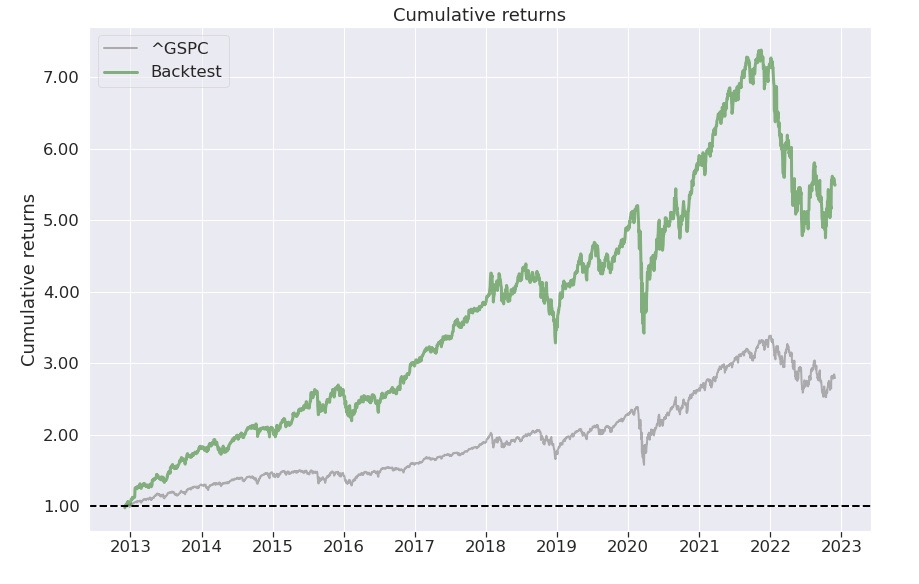
\includegraphics[width=1\linewidth]{normalTearSheet.jpeg} 
\caption{1/n}
\label{fig:subim1}
\end{subfigure}
\begin{subfigure}{0.5\textwidth}
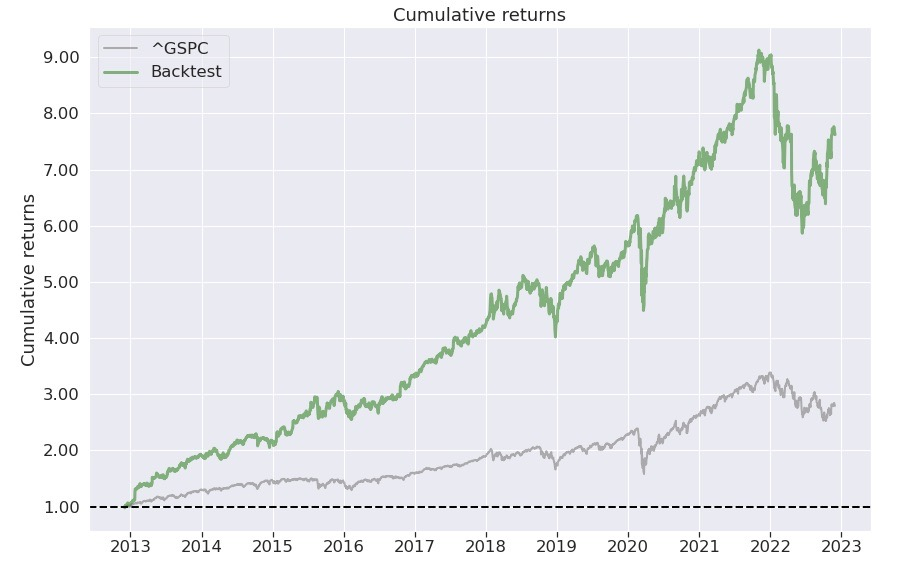
\includegraphics[width=1\linewidth]{sharpeTearSheet.jpeg}
\caption{Sharpe}
\label{fig:subim2}
\end{subfigure}
\begin{subfigure}{0.5\textwidth}
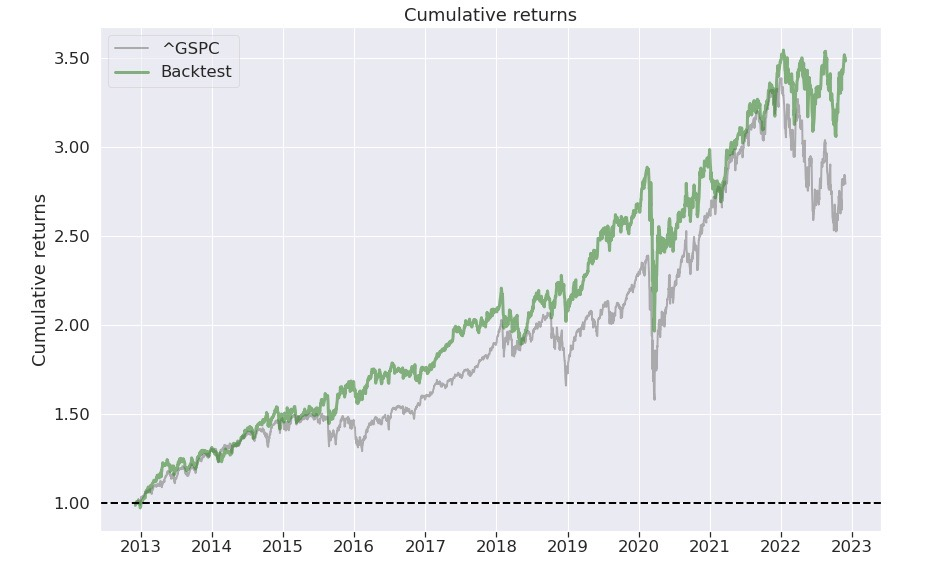
\includegraphics[width=1\linewidth]{volTearSheet.jpeg}
\caption{Volatility}
\label{fig:subim3}
\end{subfigure}

\caption{Ritorni di portafogli con pesi diversi}
\label{fig:image2}
\end{figure}

\chapter{Conclusioni}
\tableofcontents
\end{document}